\documentclass[aspectratio=169,11pt]{beamer}

% Theme based on the supplied template
\usetheme{Madrid}
\setbeamertemplate{navigation symbols}{}
\setbeamertemplate{caption}[numbered]
\setbeamertemplate{itemize items}[triangle]
\setbeamertemplate{enumerate items}[default]

\usepackage[T1]{fontenc}
\usepackage[utf8]{inputenc}
\usepackage{lmodern}
\usepackage{amsmath,amssymb}
\usepackage{booktabs,tabularx,array}
\usepackage{graphicx}
\usepackage{tikz}
\usetikzlibrary{arrows.meta,positioning,shapes.geometric,fit,calc}
\usepackage{xcolor}
\usepackage{hyperref}

% Navy/blue palette inspired by the original deck
\definecolor{TrafficNavy}{HTML}{142D52}
\definecolor{TrafficBlue}{HTML}{2678C8}
\definecolor{TrafficCyan}{HTML}{20B7C9}
\definecolor{TrafficPale}{HTML}{EAF2FB}
\setbeamercolor{structure}{fg=TrafficBlue}
\setbeamercolor{title}{fg=white,bg=TrafficNavy}
\setbeamercolor{frametitle}{fg=white,bg=TrafficNavy}
\setbeamercolor{block title}{fg=white,bg=TrafficBlue}
\setbeamercolor{block body}{fg=black,bg=TrafficPale}
\setbeamercolor{alerted text}{fg=TrafficCyan}
\setbeamertemplate{frametitle}{
  \nointerlineskip
  \begin{beamercolorbox}[wd=\paperwidth,ht=3.0ex,dp=1.15ex,leftskip=0.7cm,rightskip=0.3cm]{frametitle}
    \usebeamerfont{frametitle}\insertframetitle
  \end{beamercolorbox}
}
\setbeamertemplate{footline}{
  \leavevmode
  \hbox{
    \begin{beamercolorbox}[wd=.30\paperwidth,ht=2.6ex,dp=1.1ex,leftskip=0.4cm]{author in head/foot}
      \usebeamerfont{author in head/foot}\scriptsize TrafficSense
    \end{beamercolorbox}
    \begin{beamercolorbox}[wd=.50\paperwidth,ht=2.6ex,dp=1.1ex,center]{title in head/foot}
      \usebeamerfont{title in head/foot}\scriptsize Big Data Analytics \,|\, College of Engineering, Cherthala
    \end{beamercolorbox}
    \begin{beamercolorbox}[wd=.20\paperwidth,ht=2.6ex,dp=1.1ex,leftskip=0.4cm,rightskip=0.4cm plus 1fil]{date in head/foot}
      \usebeamerfont{date in head/foot}\scriptsize \insertframenumber/\inserttotalframenumber
    \end{beamercolorbox}
  }
}
\setbeamersize{text margin left=7mm,text margin right=7mm}
\setlength{\tabcolsep}{4pt}
\renewcommand{\arraystretch}{1.15}

\title[TrafficSense]{TrafficSense: Urban Traffic Flow Analytics \& Congestion Prediction}
\subtitle{Big Data Analytics Project}
\institute[CE Cherthala]{Department of Computer Science and Engineering\\College of Engineering, Cherthala\\[2mm]
\textbf{Faculty Guide:} Mrs.Shefna Naushad\\[2mm]}
\date{Academic Year 2026--2027}
\graphicspath{{./}{04_Results/}}  % folders LaTeX searches for images
\newcommand{\safeimg}[2][]{%
  \IfFileExists{#2}{\includegraphics[#1]{#2}}{%
    \fbox{\parbox[c][2.4cm][c]{.9\linewidth}{\centering\scriptsize
    Placeholder: \texttt{\detokenize{#2}}}}}}

\begin{document}

% 1. Title
\begin{frame}[plain]
  \titlepage
  \vspace{-0.4cm}
  \begin{center}
  \small
  \textbf{Project Team}\\[2pt]
  Abhijeet Rameshkumar Nair (CEC24AD005) \quad
  Ananthukrishna CU (CEC24AD014)\\
  Amarnath A (LCEC24AD061) \quad
  Abhinav KP (LCEC24AD058)
  \end{center}
\end{frame}

% 2. Abstract
\begin{frame}{Abstract}
\begin{columns}[T,onlytextwidth]
\column{.45\textwidth}
\begin{block}{Problem}
Traffic volume varies over time and weather. This project analyzes historical patterns, not live feeds.
\end{block}
\begin{block}{Approach}\\[7pt]
Python, Hadoop/HDFS, Hive, Spark/PySpark, and MLlib analyze Metro Interstate traffic records.
\end{block}
\column{.49\textwidth}
\begin{block}{Visualization}\\[13pt]
Hive/Spark summaries, Python plots, and Power BI communicate findings.
\end{block}
\begin{block}{Key result}
\centering \Huge \textcolor{TrafficBlue}{93.18\%}\\[-2pt]
\small chronological test accuracy for separate next-hour congestion prediction.
\end{block}
\end{columns}
\vspace{2mm}
\begin{center}
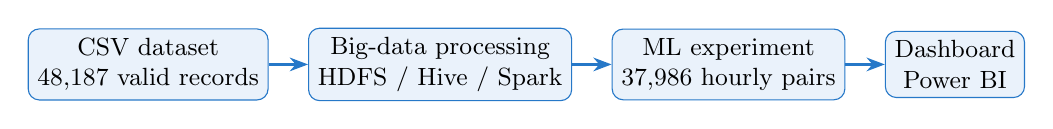
\begin{tikzpicture}[node distance=5mm, every node/.style={draw=TrafficBlue,rounded corners,fill=TrafficPale,align=center,minimum height=8mm,font=\small}]
\node (a) {CSV dataset\\48,187 valid records};
\node[right=of a] (b) {Big-data processing\\HDFS / Hive / Spark};
\node[right=of b] (c) {ML experiment\\37,986 hourly pairs};
\node[right=of c] (d) {Dashboard\\Power BI};
\draw[-{Stealth},thick,TrafficBlue] (a)--(b);
\draw[-{Stealth},thick,TrafficBlue] (b)--(c);
\draw[-{Stealth},thick,TrafficBlue] (c)--(d);
\end{tikzpicture}
\end{center}
\small The experiment used 30,388 training and 7,598 test examples.
\end{frame}

% 3. Introduction
\begin{frame}{Introduction: Why Traffic Analytics Matters}
\begin{columns}[T,onlytextwidth]
\column{.48\textwidth}
\textbf{Background}
\begin{itemize}
\item Urban traffic patterns vary throughout the day.
\item Weather and calendar conditions can coincide with changes in volume.
\item Historical records reveal recurring peak periods and congestion distributions.
\item Big Data tools support systematic organization, querying, and analysis.
\end{itemize}
\column{.49\textwidth}
\begin{block}{Problem statement}
Historical traffic records can be difficult to inspect manually. Aggregating patterns across time and weather requires a systematic workflow, while descriptive analytics alone does not test next-hour prediction. Model outputs also need validation before operational use.
\end{block}
\begin{alertblock}{Research question}
How can historical traffic data be processed and analyzed to understand congestion patterns and explore next-hour prediction?
\end{alertblock}
\end{columns}
\end{frame}

% 4. Objectives
\begin{frame}{Objectives and Project Scope}
\begin{block}{Overall objective}
Develop an integrated Big Data Analytics workflow for historical traffic analysis and congestion-prediction experimentation.
\end{block}
\begin{columns}[T,onlytextwidth]
\column{.59\textwidth}
\textbf{Objectives}
\begin{enumerate}
\item Clean and prepare the dataset.
\item Analyze time and weather patterns.
\item Use HDFS and Hive for storage and queries.
\item Run Spark processing and ML experiments.
\item Evaluate next-hour prediction chronologically.
\item Communicate findings with charts and Power BI.
\end{enumerate}
\column{.38\textwidth}
% Compact scope cards keep the second card clear of the footer.
\small
\begin{block}{In scope}
\raggedright
Historical traffic, hourly/weather patterns, congestion analysis, ML experiments, and dashboard reporting.
\end{block}
\vspace{-2mm}
\begin{alertblock}{Out of scope}
\raggedright
Live feeds, GPS route guidance, production deployment, and traffic-control actions.
\end{alertblock}
\end{columns}
\end{frame}

% 5. Literature review
\begin{frame}{Literature Review and Existing System}
\scriptsize
\begin{tabularx}{\textwidth}{>{\raggedright\arraybackslash}p{.22\textwidth} X X}
\toprule
\textbf{Author / year} & \textbf{Topic or method in presentation} & \textbf{Limitation noted} \\
\midrule
Zhu et al. (2019) & Big-data analytics in intelligent transport & Workflow integration \\
Nguyen et al. (2022) & Big-data traffic management & Conceptual analysis \\
Amini et al. (2017) & Distributed traffic-control analytics & Limited prediction \\
Maarala et al. (2015) & Spark traffic-stream analytics & Streaming emphasis \\
Jankovic et al. (2021) & ML traffic-flow prediction & Needs labelled history \\
\bottomrule
\end{tabularx}
\vspace{3mm}
\begin{columns}[T,onlytextwidth]
\column{.485\textwidth}
\begin{block}{Existing-system limitations}
Prior work may study processing, prediction, or analytics separately. Leakage can inflate a model score.
\end{block}

\hfill
\column{.485\textwidth}
\begin{block}{Project research gap}
TrafficSense links historical preparation, Hadoop/Hive, Spark experiments, and dashboard reporting; no scientific novelty is claimed.
\end{block}
\end{columns}
\footnotesize\textit{Note: Verify full bibliographic metadata for all five carried-over literature entries against the original papers.}
\end{frame}

% 6. Proposed system
\begin{frame}{Proposed System and Key Contributions}
\begin{columns}[T,onlytextwidth]
\column{.45\textwidth}
\centering
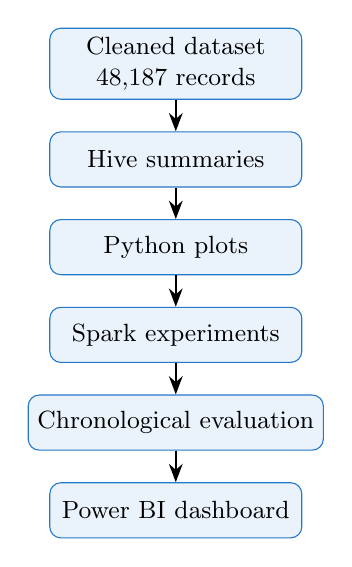
\begin{tikzpicture}[node distance=4mm, every node/.style={draw=TrafficBlue,rounded corners,fill=TrafficPale,minimum width=3.2cm,minimum height=7mm,align=center,font=\small}]
\node (a) {Cleaned dataset\\48,187 records};
\node[below=of a] (b) {Hive summaries};
\node[below=of b] (c) {Python plots};
\node[below=of c] (d) {Spark experiments};
\node[below=of d] (e) {Chronological evaluation};
\node[below=of e] (f) {Power BI dashboard};
\draw[-{Stealth},thick] (a)--(b);
\draw[-{Stealth},thick] (b)--(c);
\draw[-{Stealth},thick] (c)--(d);
\draw[-{Stealth},thick] (d)--(e);
\draw[-{Stealth},thick] (e)--(f);
\end{tikzpicture}
\column{.52\textwidth}
\begin{itemize}
\item Cleaned analytical dataset with 48,187 valid records.
\item Hive summaries for congestion, hourly traffic, and weather.
\item Python visualization scripts and stored result artifacts.
\item Spark Random Forest experimentation, including a separate next-hour task.
\item Chronological test evaluation of the next-hour experiment.
\item Power BI dashboard with historical and predicted-label distributions.
\item Actual-versus-predicted distribution comparison.
\end{itemize}
\end{columns}
\vspace{2mm}
\footnotesize\textit{Integrity note: Earlier classification was leakage-affected. The separate next-hour test accuracy is 93.18\%; dashboard distributions are not per-record validation.}
\end{frame}

% 7. Architecture
\begin{frame}{TrafficSense: Big Data System Architecture}
\centering
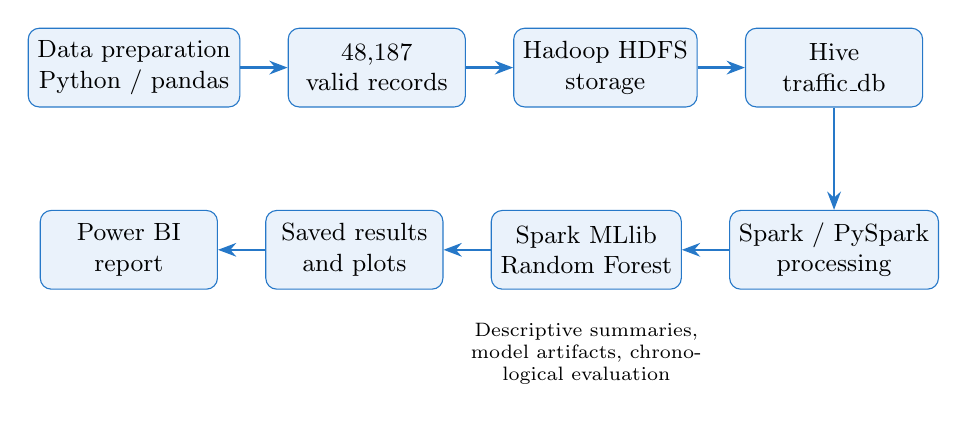
\begin{tikzpicture}[
node distance=5mm and 6mm,
stage/.style={draw=TrafficBlue,fill=TrafficPale,rounded corners,minimum width=2.25cm,minimum height=10mm,align=center,font=\small},
arrow/.style={-{Stealth},thick,TrafficBlue}]
\node[stage] (prep) {Data preparation\\Python / pandas};
\node[stage,right=of prep] (clean) {48,187\\valid records};
\node[stage,right=of clean] (hdfs) {Hadoop HDFS\\storage};
\node[stage,right=of hdfs] (hive) {Hive\\traffic\_db};
\node[stage,below=13mm of hive] (spark) {Spark / PySpark\\processing};
\node[stage,left=of spark] (ml) {Spark MLlib\\Random Forest};
\node[stage,left=of ml] (results) {Saved results\\and plots};
\node[stage,left=of results] (pbi) {Power BI\\report};
\draw[arrow] (prep)--(clean);
\draw[arrow] (clean)--(hdfs);
\draw[arrow] (hdfs)--(hive);
\draw[arrow] (hive)--(spark);
\draw[arrow] (spark)--(ml);
\draw[arrow] (ml)--(results);
\draw[arrow] (results)--(pbi);
\node[below=3mm of ml,align=center,font=\scriptsize,text width=4cm] {Descriptive summaries, model artifacts, chronological evaluation};
\end{tikzpicture}
\vspace{5mm}
\begin{block}{Architecture note}
The diagram represents the logical workflow; it does not claim a verified multi-node cluster.
\end{block}
\end{frame}

% 8. Dataset
\begin{frame}{Dataset: Metro Interstate Traffic Volume}
\begin{columns}[T,onlytextwidth]
\column{.36\textwidth}
\begin{block}{Record counts}
\begin{itemize}
\item Original: 48,204 reported records
\item Valid analytical dataset: \textbf{48,187 retained records}
\end{itemize}
\end{block}
\begin{block}{Source / format}
Kaggle dataset; CSV.\\
\url{https://www.kaggle.com/datasets/pooriamst/metro-interstate-traffic-}\\
volume\\
Date range: 2012--2018
\end{block}
\column{.61\textwidth}
\small % <--- Added to slightly reduce text size and save vertical room
\begin{tabularx}{\textwidth}{>{\raggedright\arraybackslash}p{.28\textwidth} X}
\toprule
\textbf{Feature group} & \textbf{Fields} \\
\midrule
Temporal & date\_time, year, month, day, hour, day\_of\_week \\
Weather & temp, rain\_1h, snow\_1h, clouds\_all, weather\_main, weather\_description \\
Context & holiday \\
Traffic & traffic\_volume \\
Derived target & congestion \\
\bottomrule
\end{tabularx}
\vspace{1mm} % <--- Reduced spacing from 3mm to 1mm
\begin{alertblock}{Target and geographic limits}
Categories derive from traffic-volume thresholds (exact values unavailable here). The next-hour task predicts the next hourly category. The dataset lacks road-network/GPS detail for route-specific predictions.
\end{alertblock}
\end{columns}
\end{frame}

% 9. Cleaning and EDA
\begin{frame}{Data Cleaning, Feature Engineering, and Exploratory Analysis}
\begin{columns}[T,onlytextwidth]
\column{.48\textwidth}
\begin{enumerate}
\item Start with 48,204 reported CSV records.
\item Filter the accidental header; retain 48,187 valid rows.
\item Parse time and derive calendar/weather features.
\item Derive congestion labels and prepare tables.
\end{enumerate}
\begin{block}{Next-hour pairs}
Sort by time; keep pairs exactly one hour apart; split chronologically. The 17-row difference is not confirmed duplicate removal.
\end{block}
\column{.49\textwidth}
\textbf{Schema example}
\begin{tabularx}{\textwidth}{>{\raggedright\arraybackslash}p{.42\textwidth} X}
\toprule
\textbf{Field} & \textbf{Role} \\
\midrule
date\_time & Observation time \\
traffic\_volume & Measured volume \\
weather\_main & Weather category \\
hour & Derived time feature \\
congestion & Derived label \\
\bottomrule
\end{tabularx}
\vspace{3mm}
\begin{center}
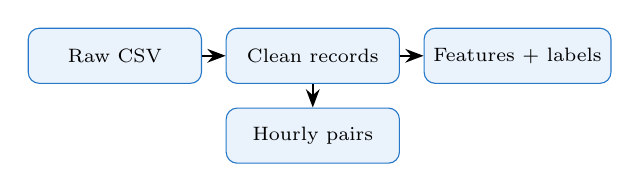
\begin{tikzpicture}[node distance=3mm, every node/.style={draw=TrafficBlue,fill=TrafficPale,rounded corners,align=center,minimum width=2.2cm,minimum height=7mm,font=\scriptsize}]
\node (a) {Raw CSV};
\node[right=of a] (b) {Clean records};
\node[right=of b] (c) {Features + labels};
\node[below=of b] (d) {Hourly pairs};
\draw[-{Stealth},thick] (a)--(b);
\draw[-{Stealth},thick] (b)--(c);
\draw[-{Stealth},thick] (b)--(d);
\end{tikzpicture}
\end{center}
\end{columns}
\end{frame}

% 10. Methodology
\begin{frame}{Methodology and Algorithm}
\begin{columns}[T,onlytextwidth]
\column{.54\textwidth}
\begin{enumerate}\itemsep0pt
\item Ingest historical dataset.
\item Clean and prepare records.
\item Store and query with HDFS / Hive.
\item Run Spark descriptive analytics.
\item Construct consecutive-hour targets.
\item Prepare features and split.
\item Train Spark MLlib Random Forest.
\item Evaluate and visualize results.
\end{enumerate}
\vspace{2mm}
\tiny \textbf{Prediction Input Variables:} current traffic\_volume, temp, rain\_1h, snow\_1h, clouds\_all, hour, day\_of\_week, month, and weather\_index.
\column{.44\textwidth}
\small
\begin{block}{Model configuration}
\begin{itemize}\itemsep-2pt
\item Random Forest ensemble
\item 50 trees, max depth: 10
\item Seed: 42
\end{itemize}
\end{block}
\begin{block}{Recorded result}
\centering \LARGE\textcolor{TrafficBlue}{93.18\%}\\
\tiny chronological held-out test accuracy
\end{block}
\end{columns}
\vspace{1mm}
\tiny Historical held-out result only, not a live metric. 
\end{frame}

% 11. Technology stack
\begin{frame}[t]{Technology Stack}
\footnotesize
\vspace{2mm}

% ---------- Row 1 ----------
\begin{columns}[T,onlytextwidth]
\column{.47\textwidth}
\begin{block}{Storage and Big Data}
\begin{minipage}[t][1.75cm][t]{\linewidth}
\begin{itemize}\itemsep0pt
\item Hadoop 3.3.6 / HDFS --- file storage.
\item Hive 3.1.3 --- SQL-like queries and table metadata.
\end{itemize}
\end{minipage}
\end{block}
\hspace{.04\textwidth}
\column{.47\textwidth}
\begin{block}{Programming and preparation}
\begin{minipage}[t][1.75cm][t]{\linewidth}
\begin{itemize}\itemsep0pt
\item Python, pandas --- data handling scripts.
\item Matplotlib --- chart generation.
\item Jupyter Notebook --- exploratory analysis.
\end{itemize}
\end{minipage}
\end{block}
\end{columns}

\vspace{4mm}

% ---------- Row 2 ----------
\begin{columns}[T,onlytextwidth]
\column{.47\textwidth}
\begin{block}{Processing and ML}
\begin{minipage}[t][1.75cm][t]{\linewidth}
\begin{itemize}\itemsep0pt
\item Spark / PySpark 3.5.1 --- data processing and experiments.
\item Spark MLlib --- Random Forest training and evaluation.
\end{itemize}
\end{minipage}
\end{block}
\hspace{.04\textwidth}
\column{.47\textwidth}
\begin{block}{Reporting and development}
\begin{minipage}[t][1.75cm][t]{\linewidth}
\begin{itemize}\itemsep0pt
\item Microsoft Power BI --- interactive dashboard.
\item Ubuntu terminal, VS Code --- environment.
\end{itemize}
\end{minipage}
\end{block}
\end{columns}

\vfill
\tiny \textit{Note: The stack reflects the recorded project environment; diagrams are logical.}
\end{frame}

% 12. Implementation
\begin{frame}[fragile,t]{Implementation: Project Structure and Core Code}
\begin{columns}[T,onlytextwidth]
\column{.54\textwidth}
\textbf{Project structure}\par\vspace{-3mm}
\fontsize{5.5}{7}\selectfont
\begin{verbatim}
TrafficSense_Project/
|-- 01_Dataset/
|   |-- Metro_Interstate_Traffic_Volume.csv
|   `-- traffic_cleaned.csv
|-- 02_Source_Code/
|   |-- first_stage.ipynb
|   |-- spark_hive_analysis.py
|   |-- create_visualizations.py
|   |-- train_next_hour_model.py
|   `-- README.md
|-- 03_Hive_SQL/
|   |-- analysis_reference.sql
|   `-- README.md
|-- 04_Results/
|   |-- congestion_distribution.png
|   |-- feature_importance.png
|   |-- feature_importance_without_volume.csv
|   |-- next_hour_forecast_results.csv
|   |-- traffic_by_hour.png
|   `-- weather_impact.png
|-- 05_Dashboard/hello.pbix
|-- 06_Documentation/
|   |-- artifact_checklist.md
|   `-- presentation_notes.md
|-- README.md
`-- README_backup.md
\end{verbatim}
\column{.43\textwidth}
\textbf{Hive analytical query}
\begin{block}{Illustrative query purpose}
Count records grouped by congestion category from the \texttt{traffic\_db} table.
\end{block}
\textbf{HDFS snippet}
\begin{block}{Recorded terminal workflow}
Start HDFS services and inspect the filesystem using HDFS commands.
\end{block}
\vfill
\footnotesize Reconstructed scripts need validation; chart, SQL, notebook, dashboard, and forecast artifacts are included.
\end{columns}
\end{frame}

% 13. Testing
\begin{frame}[t]{Testing, Validation, and Integrity Checks}
\vspace{1mm}
\scriptsize
\begin{tabularx}{\textwidth}{>{\raggedright\arraybackslash}p{.22\textwidth} X X}
\toprule
\textbf{Test} & \textbf{Expected result} & \textbf{Recorded outcome} \\
\midrule
Dataset cleaning & Filter accidental header & 48,187 valid records retained \\
Hive aggregation & Count labels & High 11,353; Low 15,216; Medium 21,618 \\
Hourly analysis & Aggregate by hour & Hourly averages available \\
Weather analysis & Aggregate by condition & Summary available \\
Next-hour preparation & Keep 1-hour pairs & 37,986 examples \\
Chronological split & Preserve time order & 30,388 train; 7,598 test \\
Model evaluation & Test held-out data & 93.18\% historical accuracy \\
Dashboard & Show summaries and labels & Existing project visualization PBIX \\
\bottomrule
\end{tabularx}

\vspace{4mm}

\begin{columns}[T,onlytextwidth]
\column{.475\textwidth}
\begin{block}{Validation strategy}
\begin{minipage}[t][1.5cm][t]{\linewidth}
\footnotesize
Use a time-ordered holdout; keep future observations out of training and separate test metrics from dashboard counts.
\end{minipage}
\end{block}
\column{.05\textwidth}
% empty spacer column: creates the gap between the boxes
\column{.475\textwidth}
\begin{alertblock}{Integrity checks}
\begin{minipage}[t][1.5cm][t]{\linewidth}
\footnotesize
Distribution bars are not a confusion matrix; \\precision, recall, and F1 values were not supplied.
\end{minipage}
\end{alertblock}
\end{columns}
\end{frame}

% 14. Results
\begin{frame}[t]{Results: Historical Traffic Patterns and ML Experiment}
\vspace{-1mm}
\begin{columns}[T,onlytextwidth]
\column{.30\textwidth}
\begin{block}{Model result}
\centering
{\fontsize{26}{28}\selectfont\textcolor{TrafficBlue}{93.18\%}}\\[-1pt]
\scriptsize chronological test accuracy
\end{block}
\vspace{-1mm}
\footnotesize
\textbf{Split}
\begin{itemize}\itemsep0pt\parskip0pt\topsep0pt
\item 30,388 train
\item 7,598 test
\item Split: 2017-11-16 20:00
\end{itemize}
\textbf{Model:} Random Forest, 50 trees, depth 10.
\column{.03\textwidth}
\column{.65\textwidth}
\textbf{\small Actual vs. predicted category counts}
\begin{center}
\footnotesize
\begin{tabular}{lrr}
\toprule
\textbf{Category} & \textbf{Actual} & \textbf{Predicted} \\
\midrule
Low & 15,216 & 14,971 \\
Medium & 21,618 & 22,461 \\
High & 11,353 & 10,755 \\
\bottomrule
\end{tabular}
\end{center}
\vspace{-1mm}
\footnotesize
More predicted Medium; fewer Low and High. Distribution comparison only, not per-record correctness.
\end{columns}

\vfill
\begin{block}{Historical data snapshot}
\scriptsize
48,187 records; average volume $\approx 3.26$K; peak $\approx 7$K. Hourly averages: 15: 5,240.46; 16: 5,663.76; 17: 5,310.08. Category averages: High 5,751.82; Medium 3,685.86; Low 794.55.
\end{block}
\vspace{1mm}
\end{frame}

% 15. Demonstration
\begin{frame}[t]{Working Demonstration: From Data to Dashboard}
\vspace{-1mm}
\begin{columns}[T,onlytextwidth]
\column{.56\textwidth}
\small
\begin{enumerate}\itemsep1pt
\item Initialize Hadoop/HDFS: start services; verify availability.
\item Verify artifacts: check recorded paths; do not assume availability.
\item Demonstrate Hive: open \texttt{traffic\_db}; run the count query if connected.
\item Show Spark/ML: present saved results and the chronological split.
\item Show Power BI: review KPIs, hourly, weather, and label views.
\end{enumerate}
\column{.41\textwidth}
\centering
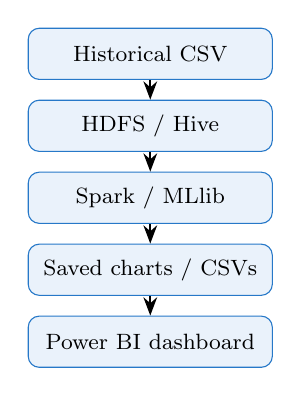
\begin{tikzpicture}[node distance=2.5mm, every node/.style={draw=TrafficBlue,fill=TrafficPale,rounded corners,align=center,minimum width=3.1cm,minimum height=6.5mm,font=\footnotesize}]
\node (a) {Historical CSV};
\node[below=of a] (b) {HDFS / Hive};
\node[below=of b] (c) {Spark / MLlib};
\node[below=of c] (d) {Saved charts / CSVs};
\node[below=of d] (e) {Power BI dashboard};
\draw[-{Stealth},thick] (a)--(b);
\draw[-{Stealth},thick] (b)--(c);
\draw[-{Stealth},thick] (c)--(d);
\draw[-{Stealth},thick] (d)--(e);
\end{tikzpicture}
\end{columns}

\vfill
\begin{alertblock}{Fallback}
\footnotesize
If services fail, present saved charts, CSVs, or the dashboard PBIX as saved project outputs.
\end{alertblock}
\vspace{2mm}
\end{frame}

% 16. Contributions
\begin{frame}[t]{Team Contributions}
\vspace{1mm}
\footnotesize

% ---------- Row 1 ----------
\begin{columns}[T,onlytextwidth]
\column{.475\textwidth}
\begin{block}{Abhijeet Rameshkumar Nair\\\scriptsize CEC24AD005}
\begin{minipage}[t][1.5cm][t]{\linewidth}
Primary technical implementation, system architecture, and project integration.\\
\textit{Support:} dataset preprocessing and feature \\engineering.
\end{minipage}
\end{block}
\column{.05\textwidth}
\column{.475\textwidth}
\begin{block}{Ananthukrishna CU\\\scriptsize CEC24AD014}
\begin{minipage}[t][1.5cm][t]{\linewidth}
Literature survey and dataset selection support.\\
\textit{Support:} presentation preparation and \\documentation.
\end{minipage}
\end{block}
\end{columns}

\vspace{3mm}

% ---------- Row 2 ----------
\begin{columns}[T,onlytextwidth]
\column{.475\textwidth}
\begin{block}{Abhinav KP\\\scriptsize LCEC24AD058}
\begin{minipage}[t][1.5cm][t]{\linewidth}
Visualization, dashboard development, and analysis support.\\
\textit{Support:} testing assistance.
\end{minipage}
\end{block}
\column{.05\textwidth}
\column{.475\textwidth}
\begin{block}{Amarnath A\\\scriptsize LCEC24AD061}
\begin{minipage}[t][1.5cm][t]{\linewidth}
Testing support and documentation.\\
\textit{Support:} project review assistance.
\end{minipage}
\end{block}
\end{columns}

\vfill
{\tiny Team collaboration included dataset selection, architecture reviews, project integration, and presentation milestones. Contributions are represented by the roles in the progress presentation; this does not imply identical coding responsibilities.}
\vspace{1mm}
\end{frame}

% 17. Conclusion
\begin{frame}[t]{Conclusion, Limitations, and Future Scope}
\vspace{-1mm}
\footnotesize
\begin{block}{Achievements}
TrafficSense demonstrates a historical-data workflow across preparation, Hadoop/Hive, Spark/ML, and Power BI. The project produced hourly and weather summaries, a dashboard of label distributions, and a separate next-hour Random Forest experiment with 93.18\% chronological test accuracy.
\end{block}

\vspace{2mm}

\begin{columns}[T,onlytextwidth]
\column{.475\textwidth}
\begin{alertblock}{Limitations}
\begin{minipage}[t][2.7cm][t]{\linewidth}
\begin{itemize}\itemsep0pt\parskip0pt\topsep0pt
\item Historical observations only; no live feeds.
\item Limited road-network and GPS detail.
\item 93.18\% historical accuracy is not live performance.
\end{itemize}
\end{minipage}
\end{alertblock}
\column{.05\textwidth}
\column{.475\textwidth}
\begin{block}{Future scope}
\begin{minipage}[t][2.7cm][t]{\linewidth}
\begin{itemize}\itemsep0pt\parskip0pt\topsep0pt
\item Evaluate precision, recall, F1, and confusion matrix.
\item Compare with suitable baseline models.
\item Add broader data and geographic information.
\item Explore sensors/GPS, Kafka, or streaming; deploy only after validation.
\end{itemize}
\end{minipage}
\end{block}
\end{columns}
\end{frame}

% 18. References
\begin{frame}{References \& Questions}
\begin{columns}[T,onlytextwidth]
\column{.68\textwidth}
\small
\begin{enumerate}
\item Metro Interstate Traffic Volume dataset. Kaggle.\\
\url{https://www.kaggle.com/datasets/pooriamst/metro-interstate-traffic-volume}
\item Apache Hadoop official documentation.
\item Apache Hive official documentation.
\item Apache Spark official documentation, including MLlib.
\item Microsoft Power BI official documentation.
\item Breiman, L. (2001). ``Random Forests.'' \textit{Machine Learning}, 45, 5--32.
\item Zhu et al. (2019); Nguyen et al. (2022); Amini et al. (2017); Maarala et al. (2015); Jankovic et al. (2021). Literature-review entries from the earlier project presentation; metadata to verify.
\end{enumerate}
\column{.29\textwidth}
\begin{center}
\vspace{1cm}
{\Huge\textcolor{TrafficBlue}{Thank You}}\\[4mm]
{\large Questions and Discussion}\\[8mm]
\textbf{TrafficSense}
\end{center}
\end{columns}
\end{frame}

\end{document}